\chapter{Conclusion}
Dans ce mémoire, nous avons exploré deux méthodes statistiques basées sur l'apprentissage machine profond et
utilisées pour la reconstruction d'image dans le contexte des lentilles gravitationnelles de type galaxie-galaxie.
Les auto-encodeurs variationnels sont utilisés pour modéliser la distribution implicite marginale d'un 
ensemble de données. Cette modélisation nous permet non seulement d'augmenter la taille de l'ensemble 
de données d'entraînement d'une machine à inférence récurentielle, mais nous permet aussi d'approximer 
une distribution de probabilité conditionnelle à une reconstruction approximative d'une galaxie 
en arrière-plan ou d'une distribution de masse d'une galaxie en avant-plan par notre modèle d'inférence. 
Cette propriété est utilisée pour le réglage fin de la machine à inférence récurentielle.

Les machines à inférence récurentielle sont utilisées pour apprendre un algorithme d'optimisation avec une convergence 
très rapide ($T \sim 10$ itérations)
en encodant des biais inductifs dans les poids d'un réseau de neurones convolutif récurrent avec une architecture U-net. 
Cette approche nous permet de préserver l'information à différentes échelles spatiales et de contrôler indépendamment 
la reconstruction à ces différentes échelles. Pour le problème inverse étudié dans ce mémoire, cette propriété s'avère cruciale. 
Finalement, pour stabiliser l'entraînement du modèle $g_\varphi$, nous avons trouvé qu'ajouter l'observation 
en entrée au modèle nous permettait d'inclure l'inférence de la valeur initiale dans la relation de récurrence. 
%Étant 
%donné le cadre théorique développé en introduction, j'interprète que ce changement permet de mieux contrôler la constante de
%Lipschitz de la machine à inférence récurentielle.

Ce travail est à la fois pertinent pour les objectifs scientifiques mentionnés en introduction, soit la recherche et l'étude 
de halos de matière noire froide et l'étude des galaxies jeunes par l'effet de grossissement des lentilles gravitationnelles, 
et aussi opportun étant donné le nombre grandissant de ces objets qu'on anticipe de découvrir dans la prochaine décennie et 
le pouvoir de résolution grandissant des grands observatoires. Mes objectifs de recherche, suivant ces succès initiaux, sont maintenant 
d'améliorer la méthode pour atteindre la résolution de télescopes comme le télescope spatial James Webb ou encore le télescope 
géant européen. Ayant démontrer que notre approche peut reconstruire un large ensemble de lentilles 
gravitationnelles simulées dans le chapitre \ref{chap:censai}, l'étape suivante pour atteindre cet objectif consiste 
à appliquer notre 
méthode à un ensemble de données provenant du téléscope spatial Hubble. 
Le fer à cheval cosmique, montrée à la figure \ref{fig:sdssj1148}, est un exemple 
particulièrement intéressant pour ce test étant donné les difficultés inhérentes a modéliser 
cette lentilles par les méthodes traditionnelles \citep{James2018,Schuldt2019,Cheng2019}.

%Des tests récents de nos méthodes montrent que 
Notre tentative récente de modéliser ce système, montrée à la figure \ref{fig:horseshoe}, indique  
déjà des résultats prometteurs. L'image de la protogalaxie en arrière-plan reconstruite avec la machine à inférence 
récurentielle possède les même 4 régions brillantes avec un taux de formation d'étoile très élevées identifiées par \citet{James2018}. 
Avec l'effet de lentille, on est en mesure d'imager cette protogalaxie avec une résolution deux fois meilleure que la 
résolution du téléscope Hubble. De plus, la distribution de masse obtenue nous indique déjà que certaines asymétries importantes, 
au delà des perturbations linéaires généralement admises autours d'un modèle elliptique,
sont probablement nécessaires pour accomplir une reconstruction statistiquement significative.

Mon second objectif de recherche est de développer un cadre statistique cohérent autour de méthodes 
d'inférences aussi puissantes, c.-à-d. être en mesure de modéliser correctement les incertitudes aléatoriques et épistémiques 
de nos reconstructions. Finalement, mon troisième objectif est d'appliquer les méthodes explorées dans cette thèse à d'autres problèmes 
inverses non linéaires, spécifiquement la reconstruction d'image dans le contexte de l'interférométrie par masque irrégulier, 
pour accélérer l'analyse de données et le processus de découverte scientifique en astronomie.


\begin{figure}[H]
        \centering
        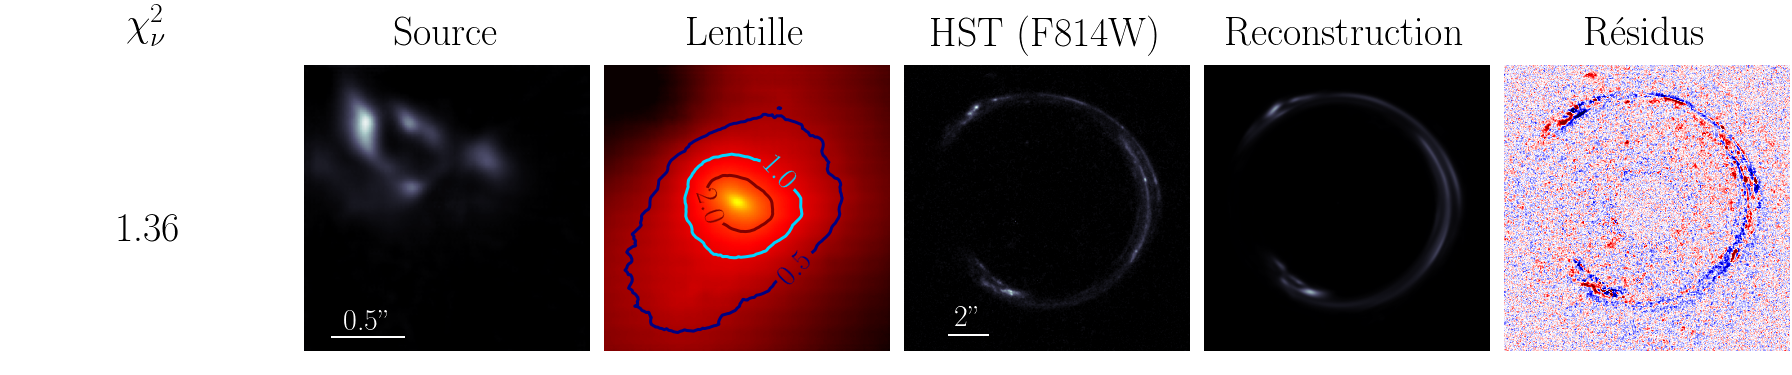
\includegraphics[width=\textwidth]{figures/horseshoe_pred2}
        \caption{Reconstruction du fer à cheval cosmique avec la machine à inférence récurentielle 
        décrite dans le chapitre \ref{chap:censai}.}
        \label{fig:horseshoe}
\end{figure}

